\subsection{Aplique lo planteado para im\'agenes en color o blanco y negro}

Se utilizará la imagen \emph{homero.bmp} en colores para realizar el trabajo.
La explicación de lo que se ha realizado en ésta pregunta es la siguiente.

(Se omitirán todas las alusiones a comandos y código, ya que aquellas se encuentran en los comentarios de los códigos generarSVD.m y descomposicionSVD.m)

\begin{itemize}
	\item Obtenemos las matrices R,G y B de nuestra imagen.
	\item Por cada matriz aplicamos SVD por separado (utilizando el algoritmo del \emph{Laboratorio I})
	\item Descomponemos cada SVD, en una suma de matrices dependiendo de sus valores propios, es decir:\\
	$U\Sigma V' = U_1 \Sigma_1 V'_1 + U_2 \Sigma_2 V'_2 + U_3 \Sigma_3 V'_3 + \ldots + U_n \Sigma_n V'_n$
	\item Cada sub SVD posee la columna n-ésima de $U$, el n-ésimo valor propio en $\Sigma$ y la n-ésima fila de $V'$
	\item Luego para poder ir probando la calidad de la imagen,
		vamos viendo la imagen para distintos $n$ valores propios:\\
		$R = \sum_{k=1}^{n}U_{R_{k}}\Sigma_{R_{k}}V'_{R_{k}}$\\
		$G = \sum_{k=1}^{n}U_{G_{k}}\Sigma_{G_{k}}V'_{G_{k}}$\\
		$B = \sum_{k=1}^{n}U_{B_{k}}\Sigma_{B_{k}}V'_{B_{k}}$
	\item Finalmente sobreponemos los nuevos R,G y B y mostramos la imagen para ver la calidad.

\end{itemize}
\newpage

\subsection{Muestre los resultados obtenidos en su informe para distintos valores de k}
\begin{center}
	\textbf{Imagen Original}\\
	
\includegraphics{img/homero}\\
\end{center}

Como nuestra imagen es de $96x96$, tendremos 96 valores propios.
	\begin{itemize}
		\item \textbf{10\ Valores\ propios}\\
			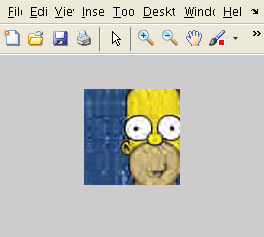
\includegraphics[height=6cm]{img/homero_10} 	
		\item \textbf{23\ Valores\ propios}\\
			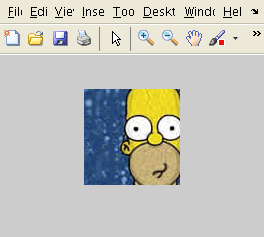
\includegraphics[height=6cm]{img/homero_23} 	
		\item \textbf{46\ Valores\ propios}\\
			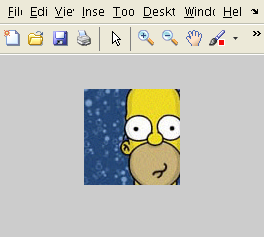
\includegraphics[height=6cm]{img/homero_46} 	
		\item \textbf{71\ Valores\ propios}\\
			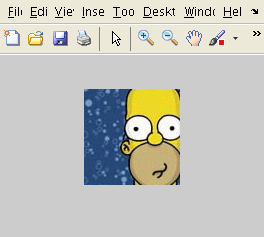
\includegraphics[height=6cm]{img/homero_71} 	
		\item \textbf{96\ Valores\ propios}\\
			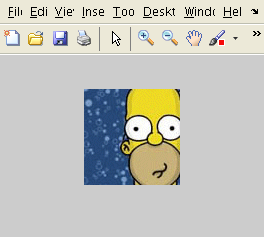
\includegraphics[height=6cm]{img/homero_96} 	
	\end{itemize}

Decidimos que con \emph{46 valores propios} ya se puede ver la imagen sin problema,
por lo tanto si pensamos que nuestra imagen es de \emph{96 valores propios} estamos realizando una reducción
de casi la mitad de valores propios, por lo cual podríamos pensar que podríamos reducir el tamaño del archivo
a la mitad, teniendo la misma información.
\newpage

\subsection{Utilizando otra factorizaci\'on, proponga otro m\'etodo para realizar el ejercicio, y concluya sobre sus resultados}

Encontramos que utilizando la factorización QR, logramos un procedimiento similar.

\begin{itemize}
	\item Obtenemos las matrices R,G y B de nuestra imagen.
	\item Por cada matriz aplicamos QR por separado.
	\item Descomponemos cada SVD, en una suma de matrices dependiendo de sus valores propios, es decir:\\
	$Q R = Q_1 R_1 + Q_2 R_2 + Q_3 R_3 + \ldots + Q_n R_n$
	\item Cada sub QR posee la columna n-ésima de $Q$ y la n-ésima fila de $R$
	\item Luego para poder ir probando la calidad de la imagen,
		vamos viendo la imagen para distintos $n$:\\
		$R = \sum_{k=1}^{n}Q_{R_{k}}R_{R_{k}}$\\
		$G = \sum_{k=1}^{n}Q_{G_{k}}R_{G_{k}}$\\
		$B = \sum_{k=1}^{n}Q_{B_{k}}R_{B_{k}}$
	\item Finalmente sobreponemos los nuevos R,G y B y mostramos la imagen para ver la calidad.
\end{itemize}

Nuevamente probaremos con distintos valores entre \emph{1 y 96}, que serian la cantidad de columnas de la matriz que ocuparemos.

	\begin{itemize}
		\item \textbf{10\ Columnas}\\
			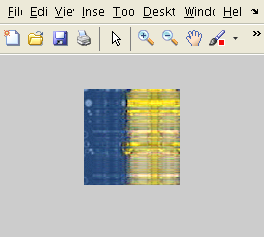
\includegraphics[height=6cm]{img/homeroQR_10} 	
		\item \textbf{23\ Columnas}\\
			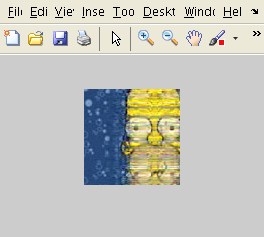
\includegraphics[height=6cm]{img/homeroQR_23} 	
		\item \textbf{46\ Columnas}\\
			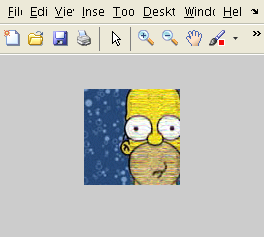
\includegraphics[height=6cm]{img/homeroQR_46} 	
		\item \textbf{71\ Columnas}\\
			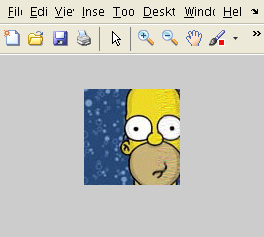
\includegraphics[height=6cm]{img/homeroQR_71} 	
		\item \textbf{96\ Columnas}\\
			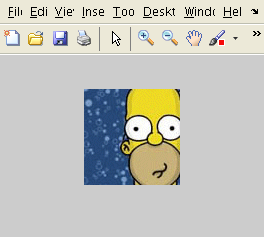
\includegraphics[height=6cm]{img/homeroQR_96} 	
	\end{itemize}

Claramente la imagen va a perdiendo calidad pero con franjas horizontales,
por lo cual es mucho mas complicado con este metodo y el 71 es mas parecido,
no como el caso anterior que con 46 valores propios funcionaba bien.
